\subsection{Dot Products}
\noindent
A dot product is a way of multiplying two vectors so that the result is a scalar.
$\vec{a}\cdot\vec{b} = \norm{\vec{a}}\norm{\vec{b}}\cos{\theta}$ where $\theta$ is the angle between $\vec{a}$ and $\vec{b}$.
One way to think of the dot product is as a measure of how much two vectors point in the same direction.
We can also show using the law of cosines that $\vec{a}\cdot\vec{b} = a_1b_1+a_2b_2+...+a_nb_n$.
Knowing the lengths of two vectors and their dot product we can calculate the angle between them as
\begin{equation*}
	\theta = \arccos{\left(\frac{\vec{a} \cdot \vec{b}}{\norm{\vec{a}} \norm{\vec{b}}}\right)}.
\end{equation*}

\begin{figure}[H]
	\centering
	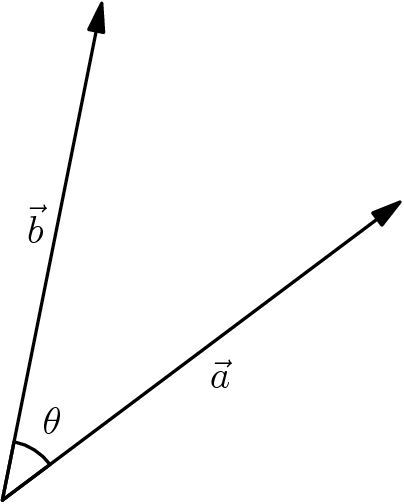
\includegraphics[width=0.25\textwidth]{../common/vectorsMatrices/DotProduct.png}
	\caption{Two vectors and the angle between them}
\end{figure}

\noindent
Although similar to scalar multiplication, dot products have some properties that set them apart.
\begin{enumerate}[label=]
	\item \textbf{Commutative}
		\begin{equation*}
			\vec{a}\cdot\vec{b} = \vec{b}\cdot\vec{a}
		\end{equation*}
		the same as scalar multiplication.
	\item \textbf{Distributive}
		\begin{equation*}
			\vec{a}\cdot\left(\vec{b}+\vec{c}\right) = \vec{a}\cdot\vec{b}+\vec{a}\cdot\vec{c}
		\end{equation*}
		the same as scalar multiplication.
	\item \textbf{\underline{NOT} Associative}
		$\left(\vec{a}\cdot\vec{b}\right)\cdot\vec{c}$ is a nonsense expression.
		However, like scalar multiplication, dot products are scalar associative.
		\begin{equation*}
			\left(c\cdot\vec{a}\right)\cdot\vec{b} = \vec{a}\cdot\left(c\cdot\vec{b}\right)
		\end{equation*}
\end{enumerate}